\documentclass[main.tex]{subfiles}
\begin{document}

\chapter{The Triplets...}

%\textbf{NL:  This chapter seems to assume a priori that the reader will be familiar with orbital dynamics and the two-body problem. Need to go through it carefully, and be sure the concepts are introduced in the right order.  But this chapter will mostly be about orbital dynamics, and the two- and three-body problems.}

%THIS CHAPTER DESCRIBES THE OUTER TRIPLE EXCITING LK OSCILLATIONS IN THE INNTER TWO BINARY COMPONENTS, EVENTUALLY CAUSING THEM TO MERGE IN A HORRIFIC AND GORY FINAL FATE.  THE NEW EMERGING SIBLING, WHILE MUCH MORE MASSIVE, IS SWEET AND KIND, AND TWEEDLEDOH IS VERY HAPPY TO MEET HIS NEW SISTER TWEEDLEDAH.
 
%Alone at last ...well, depending on how you looked at it.  
\par \nar Now gravitationally unbound from their siblings, \rmtaygete, \rmalcyone~ and \rmcelaeno~ find themselves drifting off in to the vastness of empty space.  

\section{Two's Company, Three's a Crowd}

\par \nar Three siblings alone at last.  Well, two twins and a target: the inner twins continued to gossip rudely about their outer, omni-present sister.

\par \Taygete She's a little bulbous don't you think?

\par \Alcyone  Ha ha.  Yeah, you nailed it!

\par \Celaeno  I can \textit{still} hear you two.  And I am \textit{not} bulbous.  A little round perhaps, but never bulbous.  And I shine brighter than either one of you.  So take that!

\par \Alcyone You may shine brighter than each of us individually, but together \textit{we} outshine \textit{you}.  

\par \Taygete Yeah!  Take \textit{that}!

\par \nar \rmcelaeno~ lets out a long, exasperated sigh.

\par \Celaeno My sisters, I really don't want to fight with you.  First, we're sisters from the same Mother.  Second, we're pretty much stuck together in this configuration for the next several hundred million years.  So we had might as well make the most of it.

\begin{tcolorbox}[sharp corners, colback=red!30, colframe=red!80!blue, title=Orbital Dynamics Ia]
\par \textcolor{red}{As a first approximation, the motion of celestial objects such as stars is dictated by Newton's laws of motion. These laws state that the gravitational force on a body caused by another body is determined by the masses of the two bodies, and the separation between them (decreasing with increasing distance). Something like a {\it body} may sound abstract (and a bit morbid!), but it means a point mass, that is, an object with all of its mass concentrated into a single point in space. It turns out that this is a good description if the physical object that the body represents is (close to) spherical, which is the case for most stars in the Universe. \\
To describe the motion of a system with an arbitrary number of bodies, one computes the net force on each body by adding the gravitational force from all pairs with all other bodies (known as the {\it superposition principle}). The resulting equations of motion can only be solved in closed analytic form (that is, on pen and paper) when the number of bodies is just two (one of Newton's most renowned discoveries). When the number of bodies is larger, exact solutions can only be found in specific cases. 
}
%GIVE THE READER THE LOWEST LEVEL EXPLANATION OF ORBITAL DYNAMICS POSSIBLE.}.  
\end{tcolorbox}

\begin{tcolorbox}[sharp corners, colback=blue!30, colframe=blue!80!blue, title=Orbital Dynamics Ib]
\par \textcolor{blue}{Consider two bodies with masses $m_1$ and $m_2$. Their position vectors are denoted with $\myvec{R}_1$ and $\myvec{R}_2$, respectively \note{Do we assume the reader at level blue is familiar with vectors, summation, and differentiation?}. The gravitational force on body 1 is given by
\begin{align}
\label{Chap3:Eq:F_1_vec}
\myvec{F}_{1} = - \gconst m_1m_2 \frac{\myvec{R}_1 - \myvec{R}_2}{|| \myvec{R}_1 - \myvec{R}_2||^3}.
\end{align}
\note{Have we defined $\gconst$ already by this point?} Newton's Third Law states that the force on body 2 is simply equal in magnitude but opposite in direction to that of the force on body 1, that is,
\begin{align}
\myvec{F}_{2} = - \myvec{F}_{1}.
\end{align}
If there are more than two bodies, we need to apply the superposition principle: for each pair of bodies $(i,j)$ in the system, we compute the total force on body $i$ according to
\begin{align}
\label{Chap3:Eq:GravForcei}
\myvec{F}_i = -\gconst m_i \sum_{\substack{j=1 \\ j\neq i}}^{N} m_j \frac{ \myvec{R}_i - \myvec{R}_j}{|| \myvec{R}_i - \myvec{R}_j||^3}.
\end{align}
Note that, in the summation over $j$, we must make sure that $j\neq i$, since we would otherwise double count pairs of bodies. Newton's second law for $\myvec{R}_i$ reads
\begin{align}
\label{Chap3:Eq:Newton_Second}
\myvec{F}_i = m_i \myvec{a}_i = m_i \frac{\mathrm{d}^2 \myvec{R}_i}{\mathrm{d} t^2},
\end{align}
where $\myvec{a}_i$ is the acceleration on body $i$. In Newtonian dynamics, the mass $m_i$ that appears in \Eq~(\ref{Chap3:Eq:Newton_Second}), the {\it inertial mass}, is the same as the {\it gravitational mass} $m_i$ that appears in \Eq~(\ref{Chap3:Eq:GravForcei}) (this is known as the {\it equivalence principle}). Therefore, the acceleration of body $i$ is given by
\begin{align}
\label{Chap3:Eq:EOM}
\frac{\mathrm{d}^2 \myvec{R}_i}{\mathrm{d} t^2} = - \gconst \sum_{\substack{j=1 \\ j\neq i}}^{N} m_j \frac{ \myvec{R}_i - \myvec{R}_j}{|| \myvec{R}_i - \myvec{R}_j||^3}.
\end{align}
}.  
\end{tcolorbox}

\par \Taygete \textit{Fat} chance, you bulbous sphere!

\par \Alcyone Ah ha, another good one, sister!

\par \Celaeno Well, fine.  I guess I'll take a nap then.  Better than listening to the two of you...

\section{The Demise of \rmtaygete~ and \rmalcyone}

\par \nar After some time, \rmcelaeno~ awoke from a peaceful slumber.  

\par \Celaeno Yaaaaawn... What a lovely day, wouldn't you say, \rmtaygete~ and \rmalcyone?

\par \nar \rmcelaeno~ turned her gaze toward her sisters, but was horrified by what she saw.  Her sisters' relative distance\footnote{In other words, the distance separating their respective centers of mass.} had changed over the course of their slumber.  It had gone \textit{down}, in fact.  They were now orbiting their common center of mass closer than ever before.  What's more, it seemed to \rmcelaeno that the relative angle of inclination between the inner orbital plane formed by her sisters's orbital plane and her own outer orbital plane had changed.  They were now much more coplanar than before.

%\footnote{That is, all three stars orbiting within the same 2-D plane.}  In fact, currently, \rmcelaeno~ could only see \rmalcyone~ directly; presumably, \rmtaygete~ was behind \rmalcyone, her light being eclipsed by the foreground presence of her twin sister, along the line of sight separating her from \rmcelaeno.

\begin{tcolorbox}[sharp corners, colback=red!30, colframe=red!80!blue, title=Coplanar]
\par \textcolor{red}{All objects orbit within the same 2D plane. Since there is no source of gravitational acceleration in the third dimension, isolated systems that begin coplanar will remain coplanar idenfinitely.}.  
\end{tcolorbox}

\begin{tcolorbox}[sharp corners, colback=red!30, colframe=red!80!blue, title=Orbital Inclination]
\par \textcolor{red}{DESCRIBE OR DEFINE INCLINATION OF AN ORBIT.}.  
\end{tcolorbox}

\par \nar  In fact, currently, \rmcelaeno~ could only see \rmalcyone~ directly; presumably, \rmtaygete~ was behind \rmalcyone, her light being eclipsed by the foreground presence of her twin sister, along the line of sight separating her from \rmcelaeno.

\par \nar Rather crucially, \rmtaygete~ and \rmalcyone~ now shared a much more eccentric orbit than before.

%levelone
%or leveltwo?
\begin{tcolorbox}[sharp corners, colback=red!30, colframe=red!80!blue, title=Orbital Eccentricity]
\par \textcolor{red}{The Earth orbits about the Sun on a roughly circular orbit, such that its distance from the Sun does not change much over the course of a year.  Hence, a reasonable approximation here for most purposes is that the Earth's orbital eccentricity is nearly zero, or e $\sim$ 0.  This is not the case for every orbit, however.  Some orbits have non-zero eccentricities, orbiting their centers of mass on elliptic orbits.  In the limit e $=$ 1, the two bodies orbit each along a straight line, and are doomed to crash into each other and collide for negative total orbital energies.}  
\end{tcolorbox}

\par \nar In particular, they now swung out to larger relative distances with respect to their common center of mass; here, they sit patiently due to their much slower orbital velocities. 

\begin{tcolorbox}[sharp corners, colback=red!30, colframe=red!80!blue, title=Apoastron]
\par \textcolor{red} {This part of the trajectory of an orbiting body is called ``apoastron'', and corresponds to where along an eccentric orbit the orbital velocity is at a minimum.}.  
\end{tcolorbox}

\par \nar But, they eventually swing to much closer approaches than before, their surfaces almost touching at the point of closest approach.

\begin{tcolorbox}[sharp corners, colback=red!30, colframe=red!80!blue, title=Periastron]
\par \textcolor{red}{This part of the trajectory of an orbiting body is called ``periastron'', and corresponds to where along an eccentric orbit the orbital velocity is at a maximum.}.  
\end{tcolorbox}

%levelthree:
\begin{tcolorbox}[sharp corners, colback=green!30, colframe=green!80!blue, title=Orbital Dynamics]
\par \textcolor{green}{DISCUSS ORBITAL DYNAMICS, IN THE CONTEXT OF THE TWO-BODY PROBLEM.  DESCRIBE HOW FOR STABLE TRIPLES, TO FIRST ORDER, ONE CAN APPLY THE TWO-BODY PROBLEM TWICE, TAKING THE INNER BINARY AS A SINGLE OBJECT.}.  
\end{tcolorbox}

\par \nar Each time they complete one orbital revolution, the two sisters drift a little bit closer to colliding directly with each.  On the whole, there was no mistaking the fact that their orbit was getting more compact...and fast.

\par \nar After a particularly close periastron passage, \rmtaygete~ too began to notice the changes.

\par \Taygete  Whoa!  What the hell is going on?!  I almost just collided with \rmalcyone!

\par \Alcyone Ah, yeah no kidding!  What the hell \textit{is} going on?!  Don't get so close to me the next time you pass back around...

\par \Taygete It's not like I am doing it on purpose...

\par \Celaeno  Well, don't panic just yet.  We need to figure this out, since I can't very well run off to bring back help.

\par \Alcyone Useless to the bitter end...

\par \Celaeno Cram it.  

\par \Alcyone Wait... Cram what exactly?

\par \Celaeno Your mouth.  

\par \Alcyone With what?

\par \Celaeno Anything that prevents you from talking.  

\par \Alcyone I see.  You do realize we are floating in the emptiness of an infinite vacuum, right?  It's slim pickings I am afraid, at least in so far as cramming materials are concerned.

\par \Celaeno Right, fair enough.  The point is:  stop being a jerk.  And while you are doing that, I am going to try to figure out a way to save you.  I suspect that the shift toward more co-planar orbits is directly related to the increase in your orbital eccentricity.  If you think about it, these two things in combination should conserve total angular momentum, and might arise if the components of the inner orbit spend more or less time above or below the orbital plane of the outer orbit.\footnote{Sir Isaac Newton was among the first to consider the mutual gravitational interactions of a hierarchical triple star system.  He realized that, if the orbital plane of the inner compact binary is inclined relative to the outer orbit of the tertiary companion, then an asymmetry can arise where the components of the inner binary do not spend equal amounts of time above and below the orbital plane of the tertiary.  This provides a net torque on the inner binary, reducing its orbital inclination with respect to the outer tertiary orbital plane.  In order to conserve angular momentum, the eccentricity of the inner binary must increase, reaching a maximum when the orbital plane of the inner binary crosses that of the outer tertiary.  If the eccentricity gets to be sufficiently high, then the components of the inner binary can collide and merge.  For triples that do not undergo a collision in the inner binary, these oscillations in orbital inclination and eccentricity are nowadays called "Lidov-Kozai oscillations".} 

%\footnote{DEFINE ANGULAR MOMENTUM AND CONSERVATION THEREOF.}
\begin{tcolorbox}[sharp corners, colback=red!30, colframe=red!80!blue, title=Angular Momentum]
\par \textcolor{red}{DEFINE ANGULAR MOMENTUM.}. 
\end{tcolorbox}

%LEVELTWO:
\begin{tcolorbox}[sharp corners, colback=red!30, colframe=red!80!blue, title=Conservation of Energy and Angular Momentum]
\par \textcolor{red}{DISCUSS CONSERVATION LAWS.}.  
\end{tcolorbox}

\par \nar \rmcelaeno~ finds herself lost in thought.  Several minutes pass.  Finally, an epiphany strikes.

\par \Celaeno  Wait, I've got it!  I know what is going on!

\par \Taygete  Super!  Well, please do enlighten us.

\par \Celaeno  Okay, so our unique three body configuration consists of two orbital planes.  You two orbit in one of those planes, and I orbit in another about our mutual center of mass along with the center of mass corresponding to the two of you.

\par \Alcyone  You lost me.

\par \Taygete Yeah, what's the point exactly?

\par \Celaeno The point is that your mutual orbital motion is such that its plane spends a net excess amount of time above or below my orbital plane.  It depends on our exact configuration, but that's the basic idea.  This is critical though, since it means that a net torque is being applied between our orbits.

%leveltwo:
%\footnote{DEFINE TORQUE!}
\begin{tcolorbox}[sharp corners, colback=blue!30, colframe=blue!80!blue, title=Torque]
\par \textcolor{blue}{DEFINE TORQUE.}.  
\end{tcolorbox}

\par \Alcyone And why should we care about that?

\par \Celaeno Well, unless I miss my guess, this will cause your orbital plane to be torqued toward mine, so that we are in the end orbiting roughly co-planar to each other.  Unfortunately, in order to conserve total angular momentum, this also causes the eccentricity of your orbital motion to increase.  

\par \Taygete  Huh?  Say that again?  How did you get so smart, anyways?

\par \Celaeno Hmmm...I don't know.  We're all different, right? 

\par \Alcyone Sure.

\par \Taygete Why not?

\par \Celaeno Okay, let's review.  Basically, I suspect that the shift toward more co-planar orbits is directly related to the increase in your orbital eccentricity, which we are clearly seeing.  If you think about it, these two things in combination should conserve the total angular momentum of our collective three-body system, and might arise naturally if the components of the inner orbit spend more time above (or below) the orbital plane of the outer orbit.  Apart from that, well, there's not much to say, really.  Your mutual periastron approach is already comparable to the sum of your radii.  And it is still decreasing due to the aforementioned effect.  And we haven't even considered tidal dissipation acting at periastron due to your \textit{extensive} radii being finite, which will only accelerate the rate of dissipation.

%leveltwo or levelthree:
%\footnote{	DESCRIBE TIDAL DISSPATION, AND EXPLAIN WHY IT IS MOST RELEVANT AT PERIASTRON AND FOR OBJECTS WITH LARGES RADII.}  
\begin{tcolorbox}[sharp corners, colback=blue!30, colframe=blue!80!blue, title=Torque]
\par \textcolor{blue}{DEFINE TIDAL DISSIPATION.}.  
\end{tcolorbox}

\par \Celaeno In short, you're about to collide with each other.  In fact, you'll probably merge.

\par \Taygete  Wait, WHAT?!

\par \Alcyone  WHAT?!

\begin{figure}
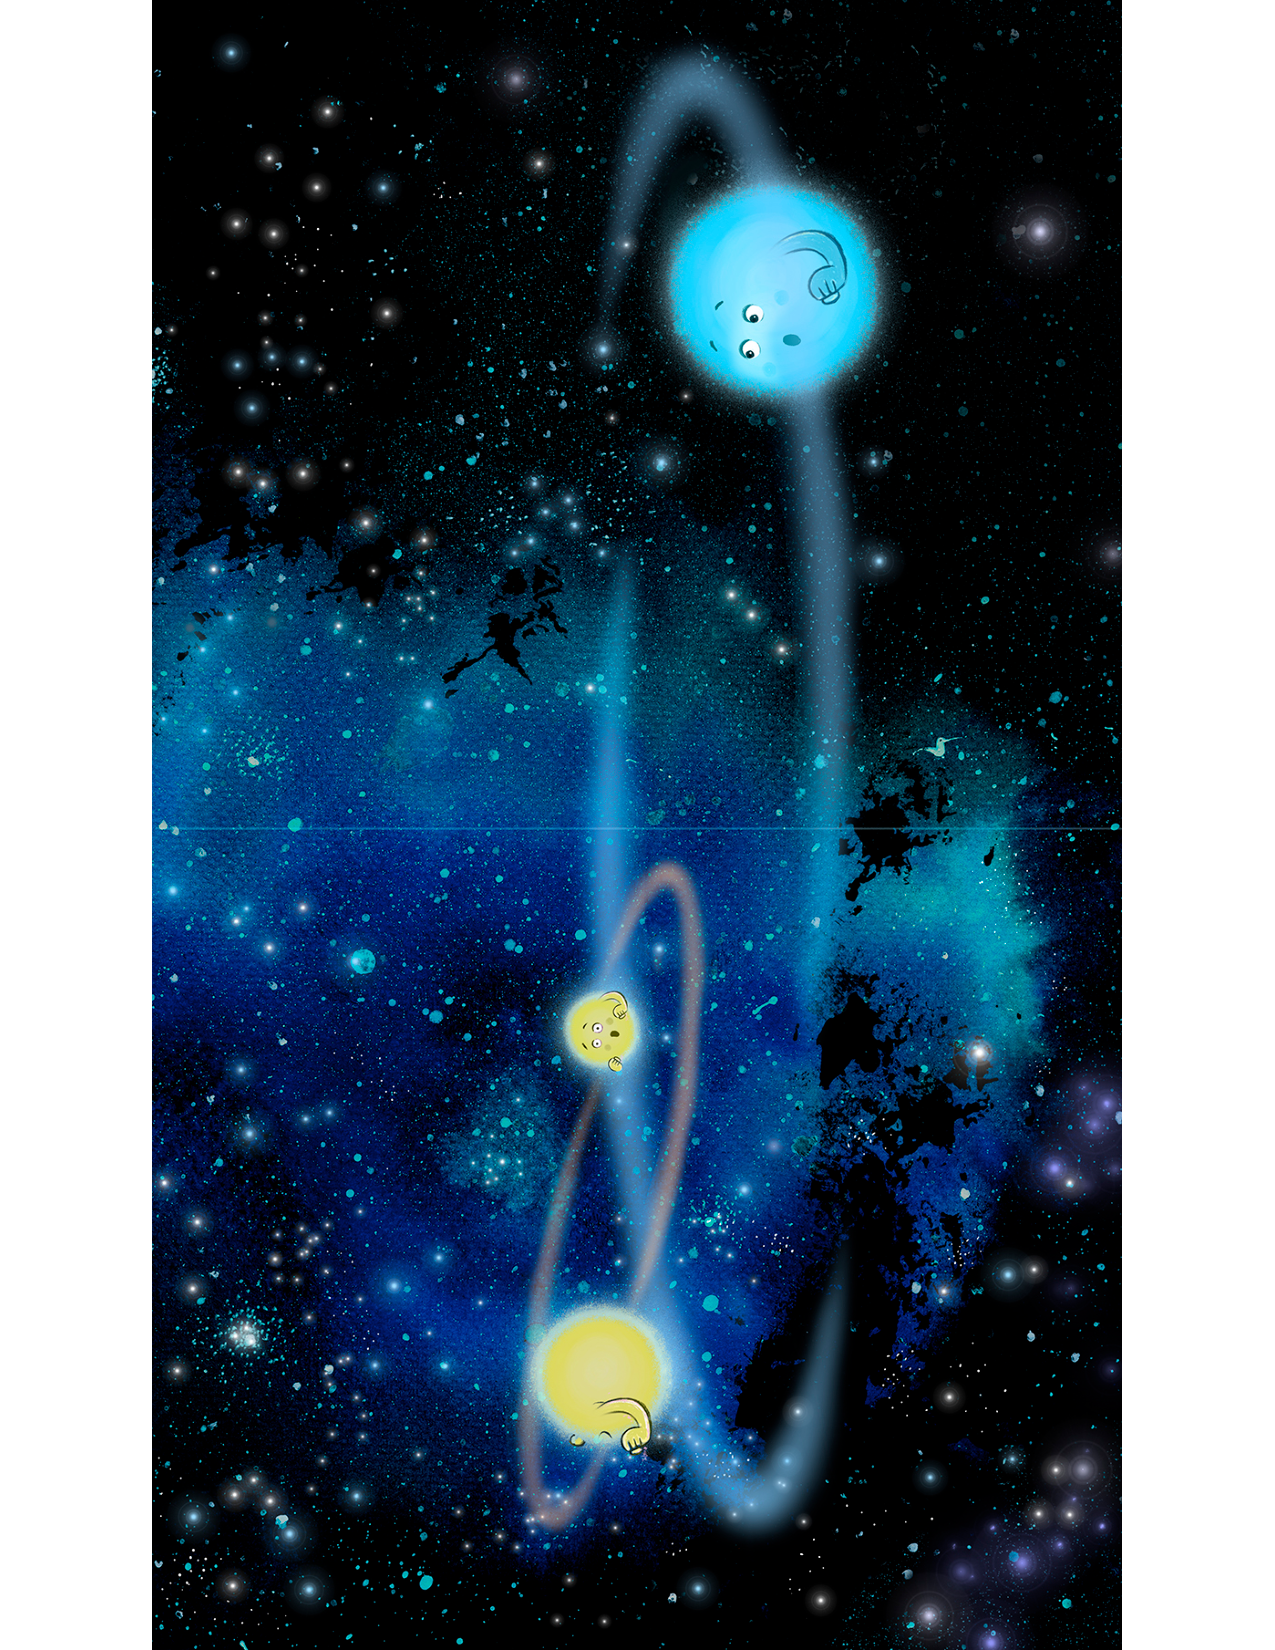
\includegraphics[width=\columnwidth,angle=270,origin=c]{ch3_1.pdf}
\caption{\rmtaygete~ and \rmalcyone, who together form the inner binary of a triple star system, after they have been informed by Celaeno that they will soon collide.  Illustration by Andre Pipe Oliva.
\label{fig:fig1}}
\end{figure}

\begin{figure}
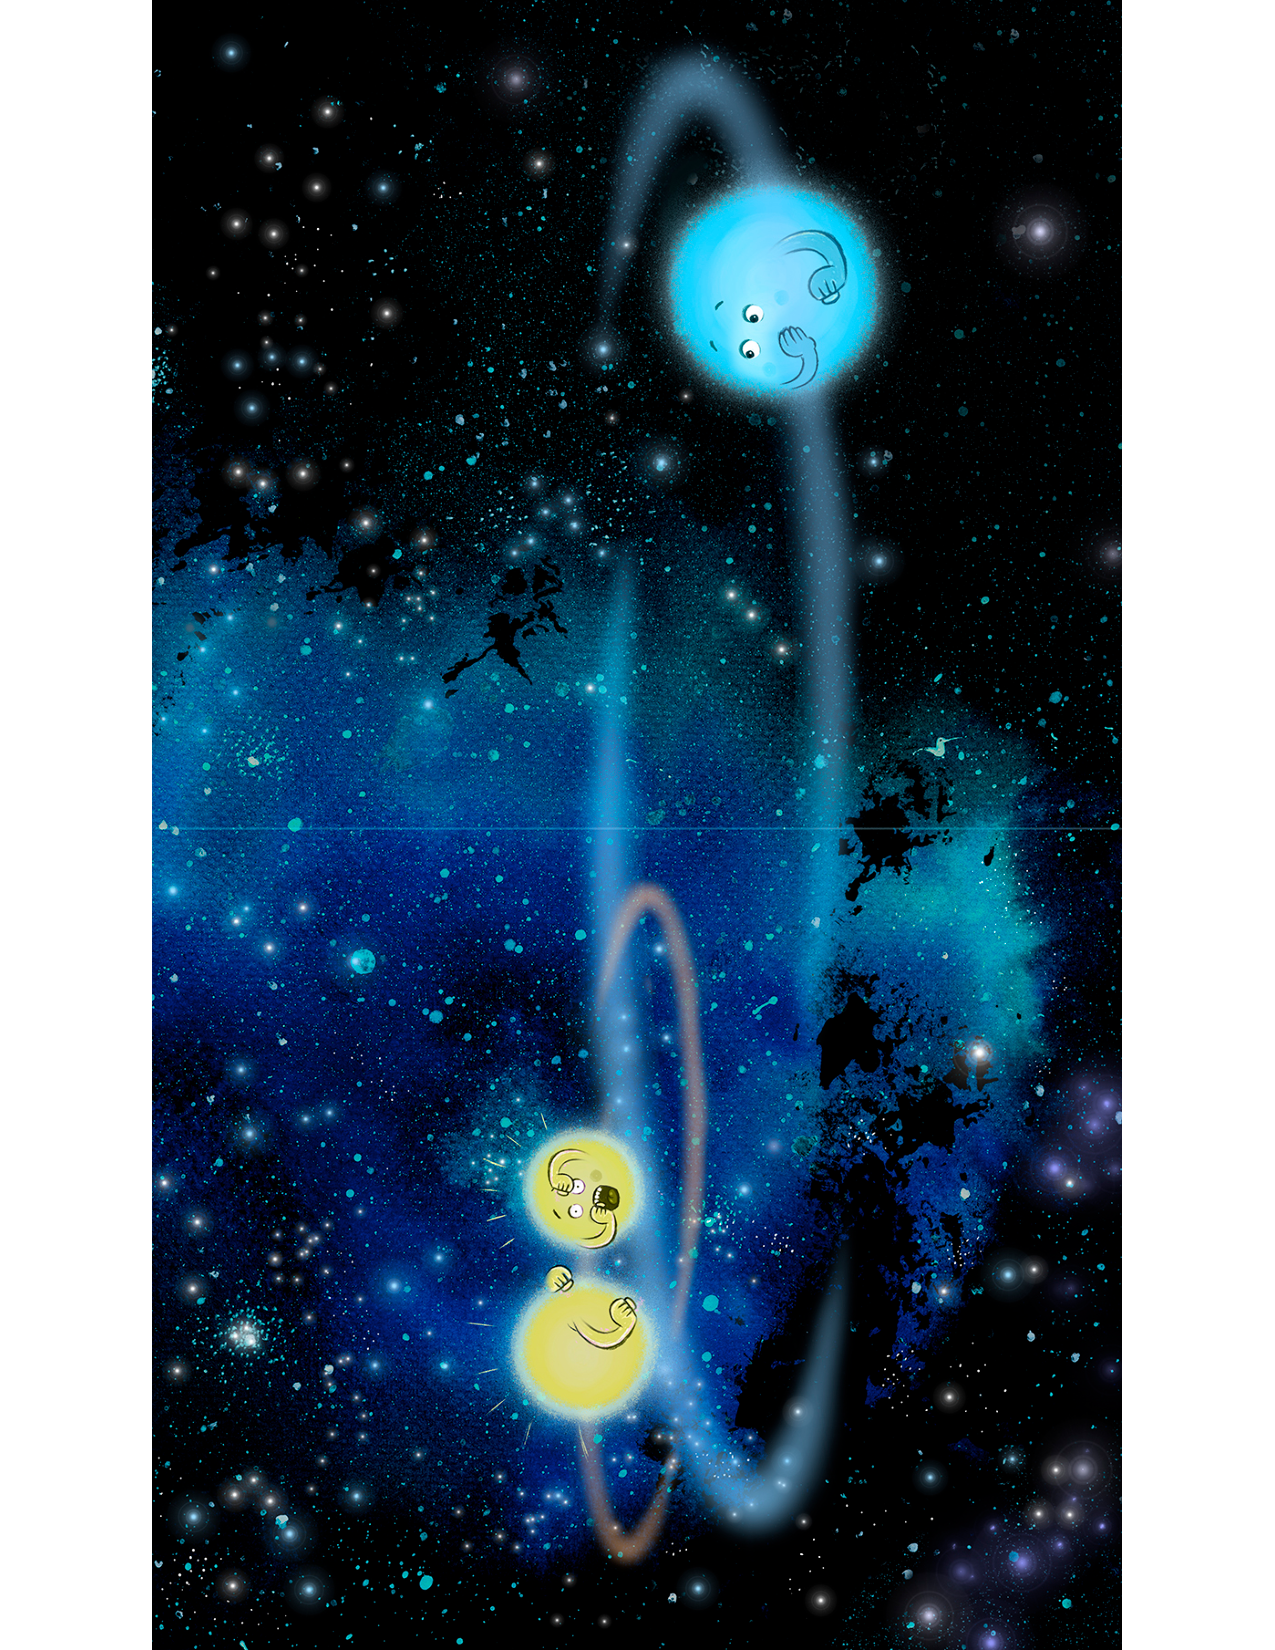
\includegraphics[width=\columnwidth,angle=270,origin=c]{ch3_2.pdf}
\caption{\rmtaygete~ and \rmalcyone, right before they collide.  Illustration by Andre Pipe Oliva.
\label{fig:fig1}}
\end{figure}

\par \nar Just then, \rmtaygete~ smashes in to \rmalcyone~ as they both re-approach their mutual periastron passage.  The collision is violent; the relative velocity is of order the sum of their local orbital speed, which is several hundred kilometers per second.  Needless to say, the sisters never stood a chance.  Their innards and organs (i.e., massive globs of hot gas) are flung violently away from the merging pair.  It is a grizzly scene.

\par \Celaeno Oh, Dear Lord!  I think I'm going to throw up.  SO MUCH PLASMA!  Gross, disgusting, and emotionally it's a lot to handle. ...Yep, here comes the vomit...

\par \nar \rmcelaeno~ suddenly vomits, spraying a particularly potent coronal mass ejection (or CME, for short) in to her immediate vicinity.  The vomited CME extends in an arc spanning about 120 degrees due to \rmcelaeno's rapid rotation rate.

\par \Celaeno Oooooooh my Gawd, they've got to be dead after that.  So gross!  

\par \nar \rmcelaeno~ nearly vomits a second time, but manages to stifle the urge.

\section{From the Ashes...} 

\par \Celaeno ...Uh...I guess I should check to see if everybody is okay? ...CAN YOU HEAR ME?!  ARE YOU STILL THERE?! 

\par \nar Gravity was in the process of taking the remains of what had once been \rmtaygete~ and \rmalcyone, and re-shaping them into a brand new star.  Formed from two stellar corpses, this new star was quickly turning out to be nearly twice as massive as each of his individual progenitors.  Suddenly, the product of this coalescence awoke.

%was spinning rapidly, but not for long; intense magnetic fields had been amplified during the collision and were rapidly spinning the new star to lower rotational frequencies.  A few millions years from now, all signs of the simultaneous deaths of two brothers, needed to give life to a new sister, will have vanished. 

\par \Lacedaemon Uh...Hello, there!  My name is...uh...\rmlacedaemon, I do believe.  I appear to be new to the scene...of which I know absolutely nothing about.  Where are we exactly?  Uh...\textit{What} are we?

\par \Celaeno Hello!  You are my new brother.  We are stars; spheres of gas and dust contracting due to gravity into the configuration you see before you, which in turn rose the temperature in our cores \textit{a lot}.  We are slowly undergoing nuclear fusion in our bellies, converting hydrogen into helium and in the process emitting energy in the form of light or photons.  The outward momentum supplied by the photons provides the outward pressure we need to balance the inward force from gravity.  Mother called it ``hydrostatic equilibrium''.

\begin{figure}
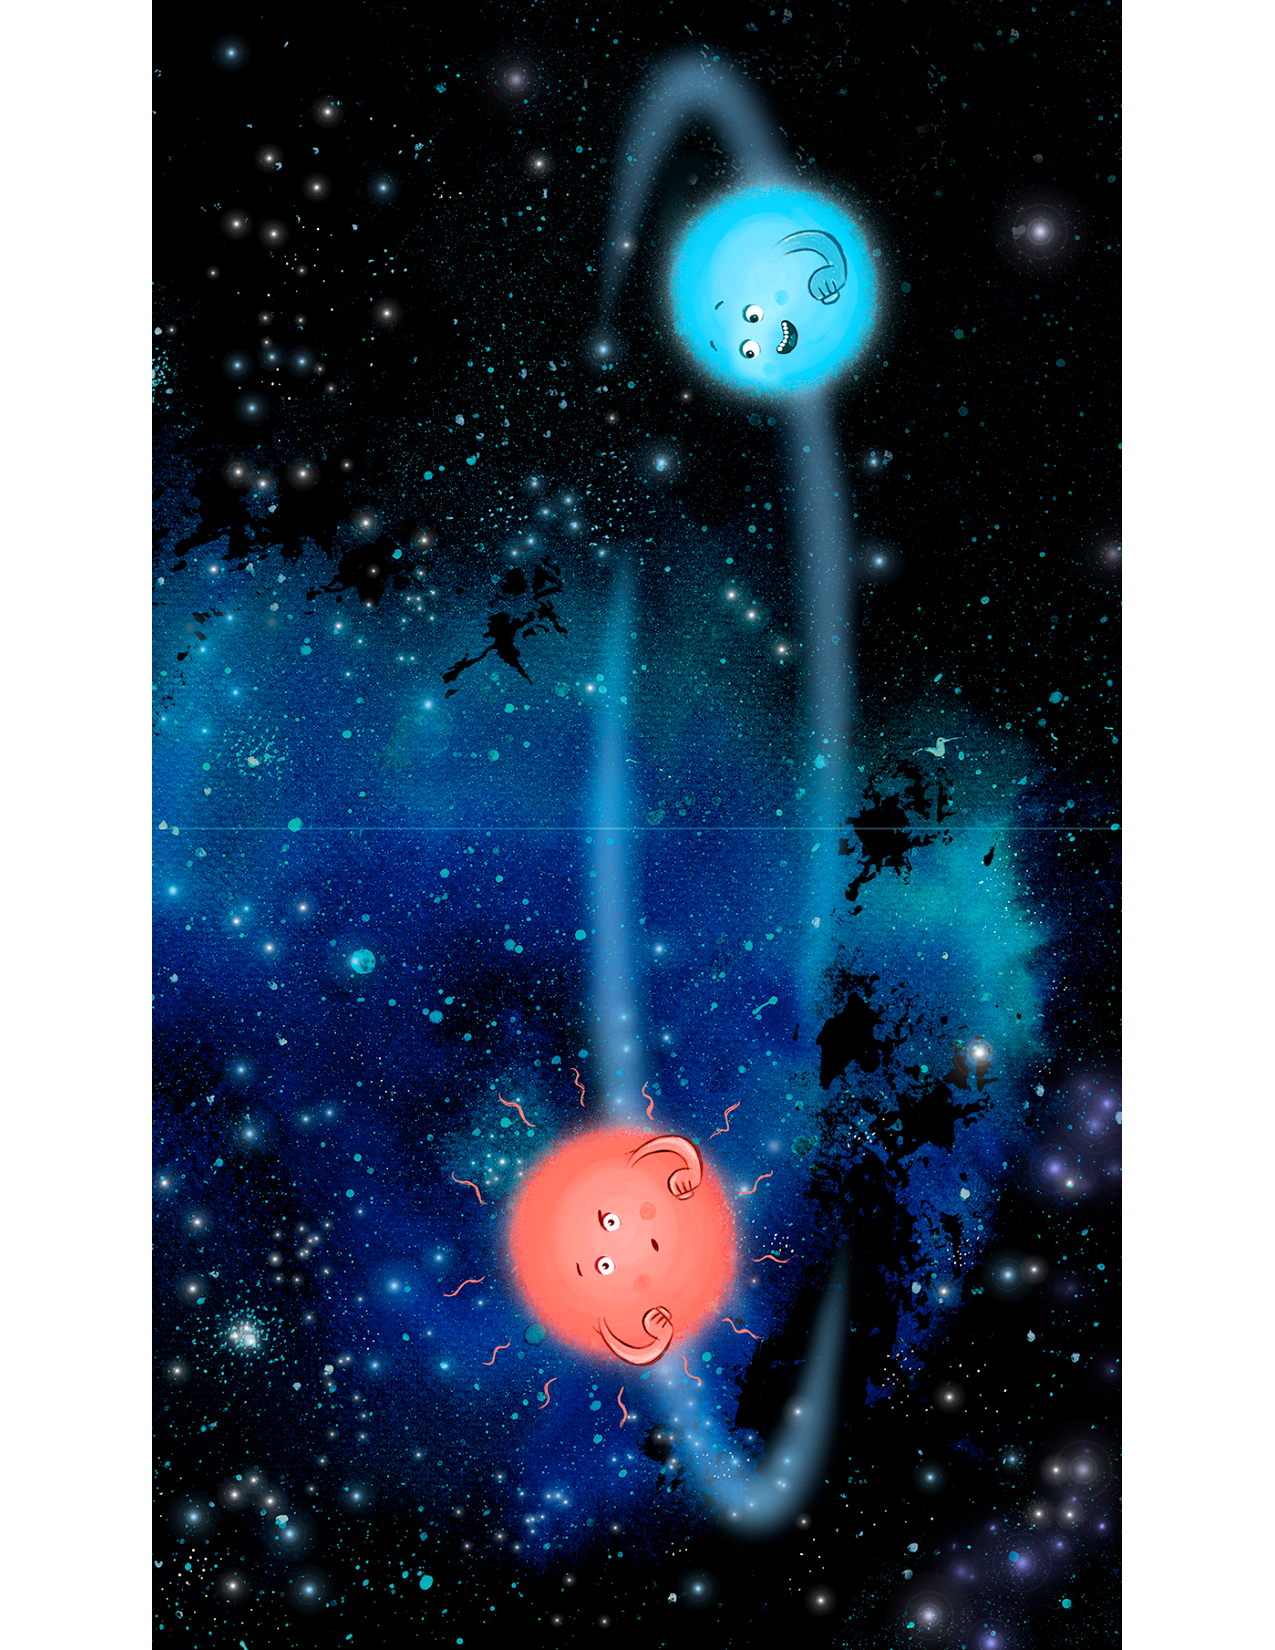
\includegraphics[width=\columnwidth,angle=270,origin=c]{ch3_3.pdf}
\caption{\rmlacedaemon~, formed from the remains of the merged \rmtaygete~ and \rmalcyone~, and his sister \rmcelaeno~.  Together, they now constitute a newly formed binary star system.  Illustration by Andre Pipe Oliva.
\label{fig:fig1}}
\end{figure}

\par \Lacedaemon Wow, that was a lot of very technical information.  Still, I appreciate it very much!  In fact, I'm quite impressed.  Now that you mention it, I'm starting to feel very balanced overall.  

\par \Celaeno I'm glad to hear it!

\par \Lacedaemon ...Well, except for this excess rotation I seem to be holding on to. And it goes right to the belly, let me tell you.  Wow, this bulge is really extending outward at my equator.  SUPER!  
%You look very svelt for a star, I must say.  I seem to be holding on to all this extra crud around my mid-center.  Rotational weight, that's the culprit.  Who would have guessed that angular momentum conservation would be this much work?

\par \nar \rmlacedaemon~ rolls his eyes to accentuate the sarcastic remark.

\par \Celaeno Don't worry, I've seen it lots of times before.  New stars spin down as they grow out of infancy.

%leveltwo or levelthree:
%\footnote{ANGULAR MOMENTUM CONSERVATION DISCUSSION, in the context of spin!}  
\begin{tcolorbox}[sharp corners, colback=blue!30, colframe=blue!80!blue, title=Torque]
\par \textcolor{blue}{DEFINE TORQUE.}.  
\end{tcolorbox}


\par \Celaeno So, the ``belly'' will go away.  You'll settle in to a more sphere-like shape in no time.  I think the whole thing has something to do with ``magnetic fields'', or so I have heard.  As near as I can tell, this is some magical force that slows your spin rate down as you mature into a beautiful new star.

\par \Lacedaemon Hey, alright!  Good news.  I'm sold.  I mean, who doesn't appreciate spherical symmetry?  Weirdos, that's who.  Uh...So now what?

\par \nar \rmcelaeno~ liked her new brother, convinced she would appreciate having him around.

\par \Celaeno We focus on the journey ahead, of course.  Who knows where our fate will take us.  But now that we are free of our siblings, I suppose almost anything \textit{could} happen.  Here is hoping for mostly good things!

\par \Lacedaemon  Wow, this is exciting!  Do you suppose we will run in to our other siblings?

\par \Celaeno Well, it's a big Galaxy out there, that much is for sure.  But, as I said, anything \textit{could} happen, especially given the long lives of stars.  

\par \Lacedaemon We have that going for us!  Wait...Just how long are we talking about?

\par \Celaeno Many millions or even billions of years.  In fact, I am guessing that somewhere out there are stars as old as the Galaxy itself.

\par \Lacedaemon Wow!  By the time I'm that old, I hope to have toured the entire Galaxy....Twice!

\par \Celaeno In that case, we had better get started.  The Galaxy sure isn't getting any smaller...

%A worried expression became evident on $\Celaeno's$ face.  
%
%\Lacedaemon  You look like you just saw something terrifying.  What's up?
%
%\Celaeno  Well, if you take our current trajectory through the Galaxy and propagate it forward through time, it looks to me like we are ultimately heading for the Galactic Center.
%
%\Lacedaemon  Great!  Wait... What is a ``Galactic Center''?
%
%\Celaeno  It is the very center of our Galaxy.  Here, a dense nuclear star cluster lives, jam packed with stars spanning all sort of masses and ages.  We are in the field of our Galaxy currently, where the mean stellar density is about 1 star per cubic parsec.  For example the distance separating the Sun and her next nearest neighbor, Proxima Centauri, is about a parsec.  But if you take the Sun and Proxima Centauri as they are observed, and drop them in to the very central regions of the nuclear cluster at the heart of our Galaxy, then more than 100 stars will fall between the pair.  The densities are that much higher.  
%
%\Lacedaemon  Wow.  That sounds crowded.  I bet you can hear \textit{everything} \textit{everyone} is doing, at any given moment.  *shudders*  
%
%\Celaeno But the really terrifying thing, if you ask me, is the super-massive black hole lurking at the heart of the nuclear cluster.    
%
%\Lacedaemon Super-massive black hole, you say?  What the hell is that?
%
%\Celaeno It is a dense dark object that does not emit light, typically way smaller than Jupter in size.  But it's total mass can range anywhere from 10$^6$ to 10$^{10}$ times the mass of the Sun.  In our own Milky Way, the super-massive black hole is known to be about 4 $\times$ 10$^6$ times the mass of the Sun.
%
%\Lacedaemon Holy cow!  That sounds....potentially violent.
%
%\Celaeno Uh... Yeah, it is.  Technically, if you wander too close to a super-massive black hole, it can eat you whole.  And, once inside its belly, you can never escape.
%
%\Lacedaemon  Oh, wonderful!  That doesn't sound even remotely terrifying...
%
%\Celaeno Um... And even if you don't get eaten, if you do wander close to a super-massive black hole, you are almost certainly going to get accelerated to extremely high velocities.  Like, we are talking thousands of kilometers per second.  
%
%\Lacedaemon  WHAT?!  Is that even possible?
%
%\Celaeno  Yep, such fast stars have definitely been seen whipping by in our very own Galaxy.  
%
%\Lacedaemon Well, this is all very terrifying.  How can we possibly prepare for a journey through the central nuclear star cluster of the Milky Way?
%
%\Celaeno Well, I'm going to take another nap, personally.  I figure we'll need to be fresh and alert, if nothing else.
%  
%
%\Lacedaemon Oh my gawd, you don't have a plan!  We are so going to die!
%
%$\Celaeno$ had already fallen asleep, and was now snoring loudly.

\end{document}

  

